\chapter{Classificazione}\label{chap:classificazione}

\section{Introduzione alla classificazione}
La \textbf{classificazione} è un altro dei problemi tipici che può essere risolto tramite un algoritmo di Machine Learning. Riguarda lo \textbf{stabilire se un dato input appartiene ad una tra delle classi} prestabilite dal problema. Il\textbf{ target non sarà più un valore} $\in \mathbb{R}$, ma una tra $k$ classi.
Per studiare la classificazione, andremo a stabilire i requisiti e i nostri obiettivi.
\begin{itemize}
	\item Un modello ben definito.
	\item Una funzione di loss per stabilire lo scarto con i risultati attesi.
	\item Un algoritmo di learning per trovare i parametri.
	\item Delle misure di valutazione.
	\item Niente overfitting!
\end{itemize}

\subsection{Classificazione: binaria e di classe}
Identifichiamo due tipi di task di classificazione:

\begin{itemize}
	\item \textbf{Classificazione binaria.}\\
	Le etichette $y \in \{ 0,1\}$. Va associata ad $x$ una delle due etichette, o le probabilità relativa a ciascuna delle due.
	\item \textbf{Classificazione di classe.}\\
	Le etichette $y \in \{ 0,1, \dots, k-1\}$. Va associata ad $x$ una delle etichette, o la probabilità relativa a ciascuna di esse. In realtà $\hat{y}$ (la predizione) è un vettore di $k$ elementi, in cui ogni elemento rappresenta la probabilità che $x$ appartenga alla classe associata a quell'elemento.
\end{itemize}

È fondamentale sottolineare l'importanza che gli output di questi algoritmi siano sempre $\in[0,1]$, in quanto da interpretare come \textbf{probabilità}.
\section{Classificazione binaria}
Nonostante i classificatori binari possano sembrare limitati, questi trovano applicazioni in vari task: solitamente, questi si basano sulla suddivisione di immagini più grandi in \textit{patches} più piccole, con una successiva, appunto, classificazione, per individuare determinati elementi. Nel \textbf{medical imaging}, i classificatori binari possono individuare piccoli tumori. Nei \textbf{controlli qualità }in ambito industriale, possono individuare \textbf{imperfezioni} nei materiali. Nel campo più generale della \textbf{computer vision}, gli algoritmi di classificazione (binaria e non) sono fondamentali.

\subsection{Perché non usare la regressione lineare per la classificazione?}

Si potrebbe pensare di \textbf{usare un modello di regressione lineare per effettuare classificazione binaria}, e l'intuizione non sarebbe nemmeno totalmente sbagliata: potremmo usare, ad esempio, la regressione per \textbf{trovare una retta che unisce i dati }in maniera opportuna, e in funzione della pendenza di questa retta, \textbf{stabilire un valore di sogliatura }per distinguere due classi.

Forniamo il seguente esempio: vogliamo addestrare un modello per prevedere se un tumore è benigno o maligno usando una singola feature (dimensione del tumore).

Usiamo la regressione lineare e facciamo il fitting di una retta nello spazio (troviamo la retta, cioè la funzione che meglio si posiziona a media tra tutti i punti). Possiamo trovare il miglior $y = \vartheta^Tx$ dal nostro set di dati e quindi selezionare una \textbf{soglia} su $y$ per classificare quando il tumore è maligno o meno:
$h_\vartheta(x) \leq 0.5 \to 0, \quad h_\vartheta(x) \geq 0.5 \to 1$.

\begin{figure}[tbph]
	\centering
	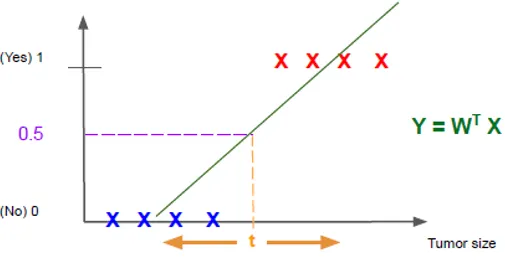
\includegraphics[width=0.7\linewidth]{images/regression-for-classification.png}
	\caption{Utilizzo della regressione lineare per classificazione binaria: viene stimata una retta $y = \vartheta^T x$ sui dati e si introduce una soglia (ad esempio $0.5$) per distinguere le due classi. I punti sotto la soglia vengono classificati come $0$ (tumore benigno), mentre quelli sopra come $1$ (tumore maligno).}
\end{figure}

Ci sono \textbf{due criticità} relative all'utilizzo della regressione. La prima, riguarda la versatilità del modello: il fitting della retta non è opportuno, in  quanto la regressione lineare dipende fortemente dalla distribuzione dei dati.


\begin{figure}[tbph]
	\centering
	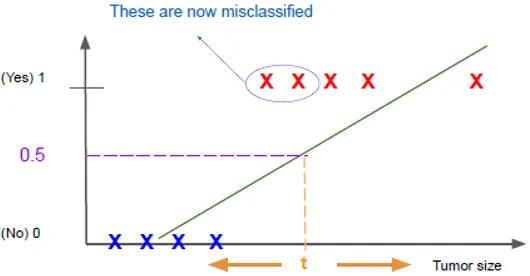
\includegraphics[width=0.7\linewidth]{images/regression-for-classification2}
	\caption{Sensibilità della regressione lineare alla distribuzione dei dati: l'aggiunta o lo spostamento di alcuni esempi modifica significativamente la retta stimata, causando errori di classificazione rispetto alla soglia fissata. Questo evidenzia una delle principali criticità dell'uso della regressione lineare per compiti di classificazione.}
\end{figure}

La seconda criticità riguarda invece la $y$, non sempre limitata tra 0 e 1, come ci aspettiamo in un modello di classificazione binaria. Come ci comportiamo con valori più grandi di 1? E con valori minori di 0? Possiamo risolvere il problema introducendo delle funzioni, dette funzioni \textbf{di linking}. Queste ci permettono di \textbf{adattare i nostri valori }a modelli di regressione che altrimenti non sarebbero opportuni per la classificazione. Vediamo un esempio relativo alla regressione logistica usando la funzione \textbf{sigmoide}.

\section{Regressione logistica - Sigmoide}
Se la regressione lineare restituisce una $y$ non limitata tra 0 e 1, la \textbf{regressione logistica} risolve il problema con una funzione, detta \textbf{sigmoide}, applicata sul risultato $z = \vartheta^TX$ del modello di regressione. La \textbf{sigmoide} una funzione del tipo

$$
\sigma(z) = \frac{1}{1 + e^{-z}} = \frac{1}{1 + e^{-\vartheta^TX}}
$$
\noindent
con $z = \vartheta^T X$. Questa funzione ha un'interpretazione probabilistica molto banale, opportuna per \textbf{adattare i modelli di regressione lineare su problemi di classificazione}\footnote{Non si può pretendere di usare un modello di regressione lineare su task di classificazione, senza fare alcun tipo di modifica, come quelle che introduciamo con la sigmoide.}. Osserviamo che:

\begin{itemize}
	\item $1-\sigma = \sigma(-z)$
	\item $\displaystyle\frac{\partial \sigma(z)}{\partial z} =\sigma(z)(1-\sigma(z)) = \sigma(z)\sigma(-z)$
	\item È inoltre dimostrabile che $\displaystyle\sigma = \frac{1}{2} + \frac{1}{2}\tanh\left(\frac{z}{2}\right)$. Questo ci apre le porte a implementazioni molto più semplici.
\end{itemize}

Da qui il modello di regressione logistica è definito come:
\[
h_\vartheta (x) = \sigma(\vartheta^T x) = \frac{1}{1 + e^{-\vartheta^T x}}
\]

\paragraph{Decision boundaries.}
Il modello di regressione logistica, come quello di regressione lineare, è un classificatore lineare. La decision boundary è definita come l'insieme dei punti per cui il classificatore è incerto, ovvero quando le probabilità restituite sono uguali per entrambe le classi (nel caso binario, quando $P(y=1|x) = P(y=0|x)$). Nella regressione logistica questo avviene quando
\[
\sigma(\vartheta^T x) = 0.5 \quad \Rightarrow \quad \vartheta^T x = 0
\]
il che porta a un decision boundary lineare definito dall'iperpiano $\vartheta^T x = 0$. I punti su questa linea rappresentano la soglia di decisione del classificatore, dove è incerto se assegnare l'etichetta $0$ o $1$.

\begin{figure}[tbph]
	\centering
	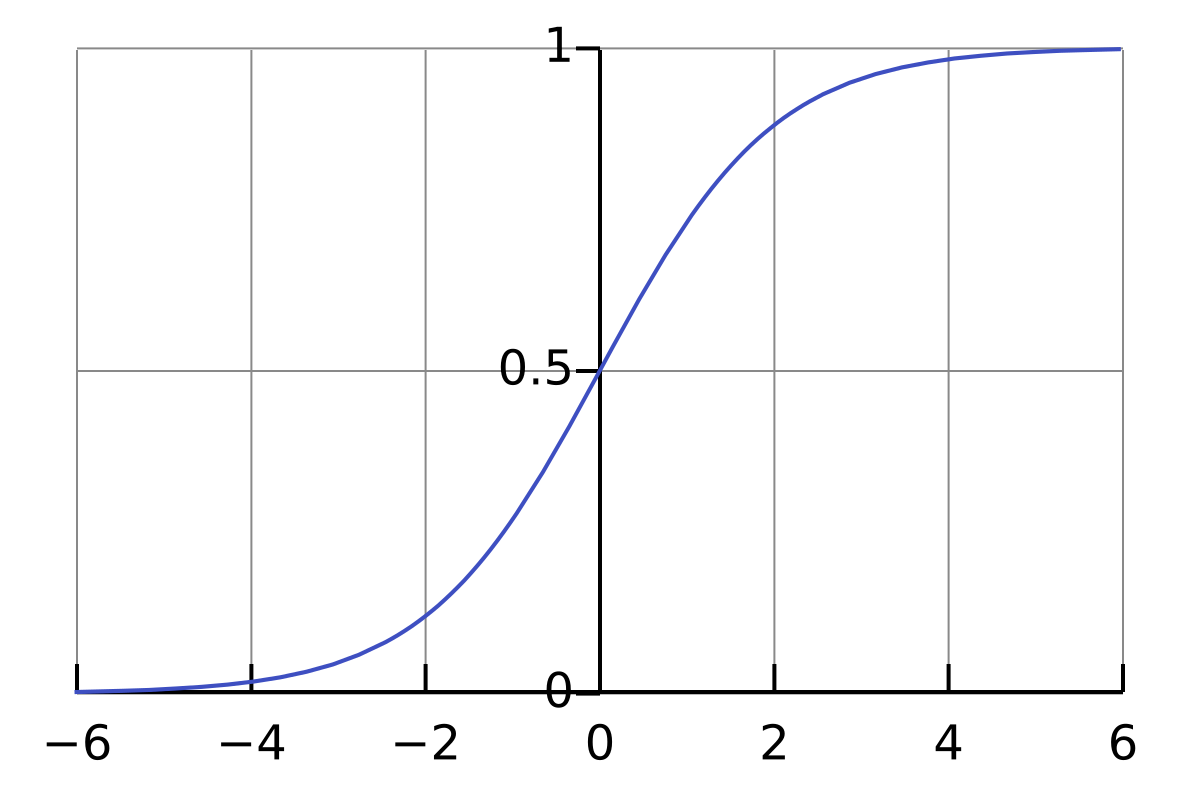
\includegraphics[width=0.6\linewidth]{images/sigmoid}
\end{figure}


\subsection{Vantaggi relativi all'uso della sigmoide}

\begin{itemize}
	\item Interpretazione probabilistica semplice. Da valori $\in[0,1]$.
	\item Derivabile, più liscia rispetto ad una step function.
	\item Introduce non lineareità, migliorando la classificazione.
\end{itemize}

\section{Funzione di Loss}

Avere una funzione di Loss associata al modello è fondamentale per definire il criterio di apprendimento e determinare i parametri $\vartheta$ ottimali per il problema di classificazione. 

Nel caso della regressione logistica, la funzione di Loss è definita in funzione della \textbf{vera etichetta} $y \in \{0,1\}$ e della predizione del modello $h_\vartheta(x)$.

Per un singolo esempio $(x,y)$, definiamo la loss come:

$$
\text{Loss}(h_\vartheta(x), y) =
\begin{cases}
- \log(h_\vartheta(x)) & \text{se } y = 1 \\[6pt]
- \log(1 - h_\vartheta(x)) & \text{se } y = 0
\end{cases}
$$

Questa definizione penalizza fortemente le predizioni errate:
\begin{itemize}
    \item se $y = 1$ e $h_\vartheta(x)$ è vicino a 0, la loss diverge;
    \item se $y = 0$ e $h_\vartheta(x)$ è vicino a 1, la loss diverge.
\end{itemize}

Possiamo riscrivere la funzione in forma compatta, sfruttando il fatto che $y$ è binaria:

$$
\text{Loss}(h_\vartheta(x), y)
=
- \left[
y \log(h_\vartheta(x)) 
+ 
(1-y)\log(1 - h_\vartheta(x))
\right]
$$

Questa espressione è equivalente alla definizione precedente ma consente una trattazione analitica più semplice, in particolare nel calcolo del gradiente.

\bigskip

Definita la loss per un singolo esempio, possiamo introdurre la \textbf{funzione di costo} (cost function), che rappresenta la media della loss su tutti i $m$ esempi del training set:

$$
J(\vartheta)
=
-\frac{1}{m}
\sum_{i=1}^{m}
\left[
y^{(i)} \log(h_\vartheta(x^{(i)}))
+
(1-y^{(i)}) \log(1 - h_\vartheta(x^{(i)}))
\right]
$$

La funzione di costo viene minimizzata tramite l'algoritmo di discesa del gradiente:

$$
\vartheta_j^{\text{new}}
=
\vartheta_j^{\text{old}}
-
\alpha
\frac{\partial J(\vartheta)}{\partial \vartheta_j}
\qquad \forall j
$$

dove $\alpha$ è il learning rate, iperparametro che controlla l'ampiezza del passo di aggiornamento.


\subsection{Derivata parziale della funzione di costo}

Necessaria per applicare la discesa del gradiente.
$$
\frac{\partial J(\vartheta)}{\partial \vartheta_j} = \frac{1}{m} \sum_{i=1}^{m} (\underbrace{h_\vartheta(x^{(i)})}_{(*)}- y^{(i)}))x_j^{(i)}) \qquad \forall j = 0, \dots, d
$$
(*) Questo membro nasconde la funzione sigmoide $\sigma(\vartheta^TX^{(i)})$.

\subsection{Entropia dell'informazione}

La funzione di loss usata nella regressione logistica (Binary Cross Entropy) ha una chiara interpretazione informativa: misura quanto la distribuzione di probabilità predetta dal modello si discosta dalla distribuzione ``vera'' delle etichette. Per introdurre questa idea, partiamo dal concetto di \textbf{entropia} di una variabile discreta, che quantifica il grado di incertezza associato a una distribuzione di probabilità.

Sia \(X\) una variabile aleatoria discreta che può assumere \(K\) valori con probabilità \(p_1,\dots,p_K\). L'entropia è definita come:
\[
H(X) = -\sum_{k=1}^{K} p_k \log_2(p_k).
\]
\noindent
Intuitivamente, l'entropia è:
\begin{itemize}
	\item \textbf{alta} quando la distribuzione è ``uniforme'' (massima incertezza);
	\item \textbf{bassa} quando la distribuzione è concentrata su pochi valori (bassa incertezza).
\end{itemize}

\noindent
Nel caso binario (\(K=2\)), con probabilità \(p_1\) e \(p_2=1-p_1\), otteniamo:
\[
H(X) = - p_1\log_2(p_1) - p_2\log_2(p_2).
\]

\begin{figure}[tbph]
	\centering
	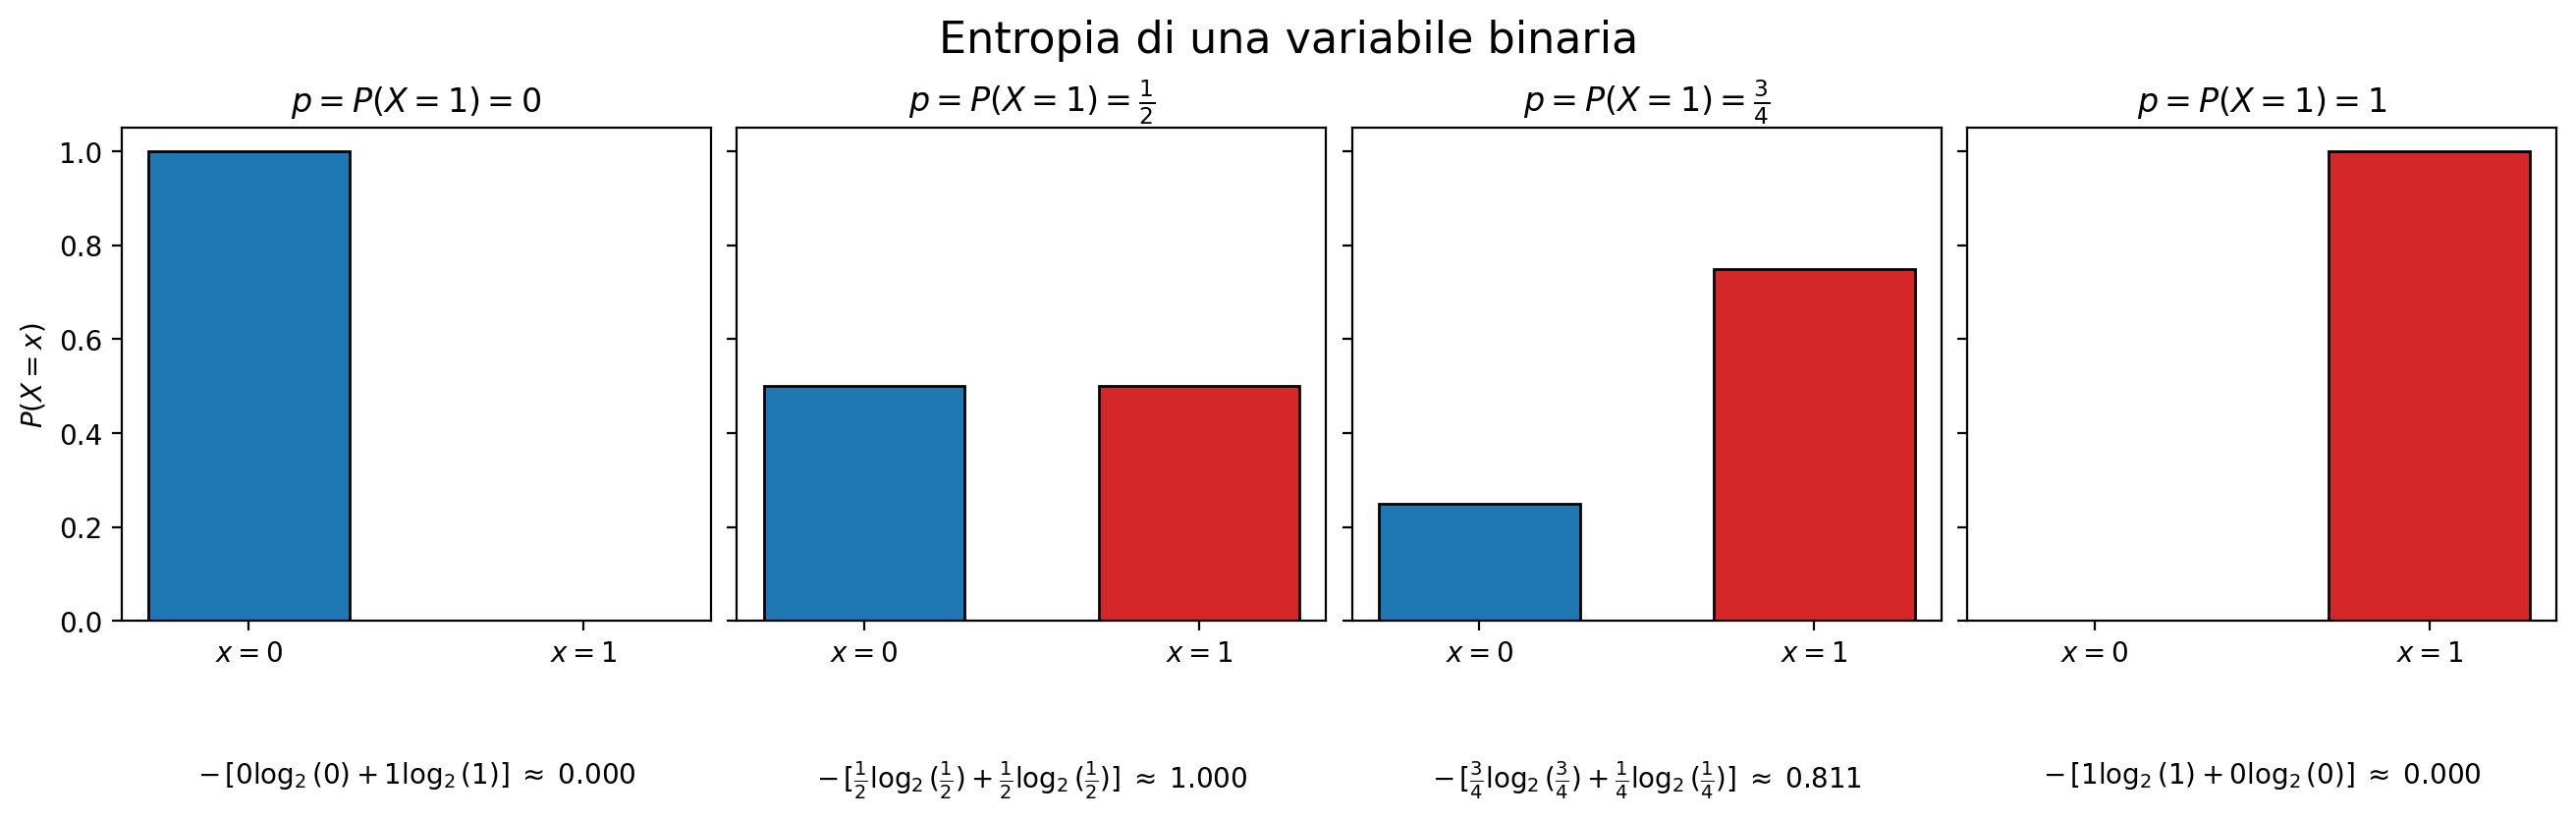
\includegraphics[width=1\linewidth]{images/entropy_sketch}
\end{figure}

\textit{NB} Il termine \(\log_2(0)\) non è definito, ma nel calcolo dell'entropia (e della cross-entropy) si usa il limite:
\[
\lim_{p\to 0^+} p\log(p)=0,
\]
per cui assegnare probabilità esattamente nulle non crea problemi teorici. In pratica, per evitare instabilità numeriche, le implementazioni ``clippano'' le probabilità in \((\varepsilon, 1-\varepsilon)\) con \(\varepsilon\) molto piccolo. Inoltre, predizioni estremamente confidenti (\(p \approx 0\) o \(p \approx 1\)) non implicano di per sé overfitting: l'overfitting riguarda la \emph{generalizzazione} (prestazioni su dati non visti), non il valore di una singola probabilità stimata.


\paragraph{Esercizio sull'entropia.}
Riordina le seguenti distribuzioni in ordine crescente di entropia.

\begin{figure}[tbph]
	\centering
	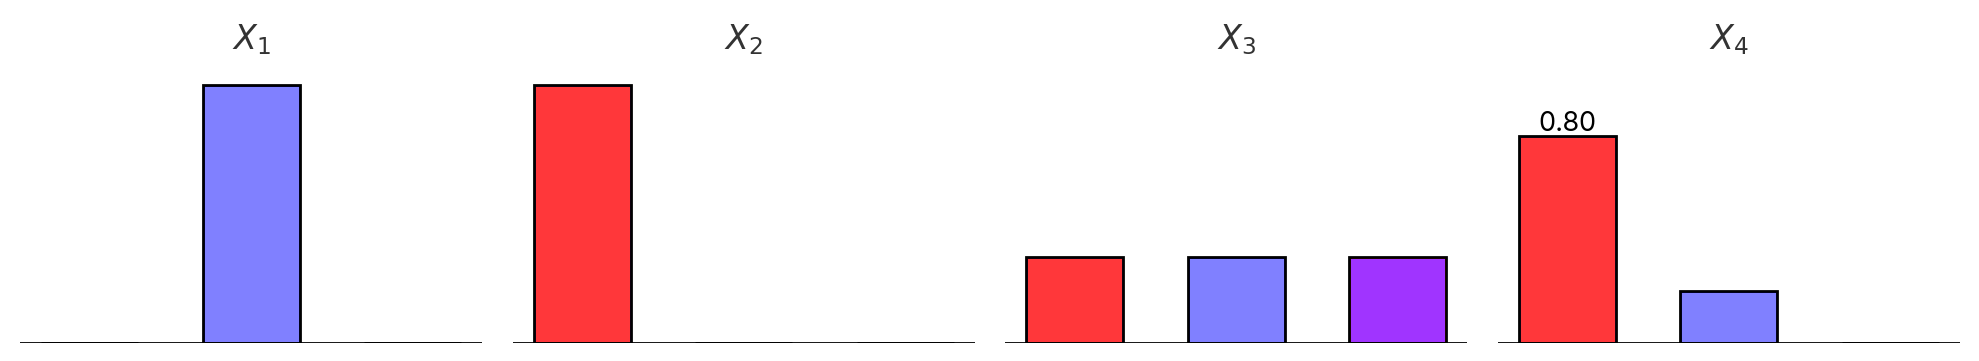
\includegraphics[width=1\linewidth]{./images/entropia-esercizio}
\end{figure}

$$
H(X) = - p_1\log_2(p_1) - p_2\log_2(p_2) = -[p_1\log_2(p_1) + p_2\log_2(p_2) + p_3\log_2(p_3) ]
$$

\begin{enumerate}
	\item $H(X_1) =  -[0\log(0) + 1\log(1) + 0\log(0) ] = 0$
	\item $H(X_2) =  -[1\log(1) + 0\log(0) + 0\log(0) ] = 0$
	\item $H(X_3) =  -[0,33\log(0,33) + 0,33\log(0,33) + 0,33\log(0,33) ] \approx 1,5848$
	\item $H(X_4) =  -[0,80\log(0,80) + 0,20\log(0,20) + 0\log(0) ] \approx 0,722$
\end{enumerate}

$$
X_1 = X_2 < X_4 < X_3
$$

\subsection{Binary Cross Entropy Loss}

La seguente formula è equivalente alla nostra funzione di Loss, ma fornisce un'interpretazione più intuitiva. Definiamo la \textbf{Binary Cross Entropy Loss} come:

$$
H_{BCE}(X) = \frac{1}{m}\sum_{i=1}^{m} \left(-\sum_{k=1}^{K}\underbrace{p_k^{(i)}}_{\text{(a)}} \log_2(\underbrace{q_k^{(i)}}_{\text{(b)}})\right)
$$

Dove (a) è la distribuzione vera della classificazione, detta \textbf{ground truth}, ovvero quella con probabilità massima sulla classe attesa, mentre (b) è la distribuzione data dal classificatore. Misura quindi la \textbf{distanza tra le due distribuzioni}. Minimizzare $H_{BCE}(X)$, significherà rendere le distribuzioni ideali e quelle effettive del classificatore, quanto più simili possibile.

\begin{figure}[tbph]
	\centering
	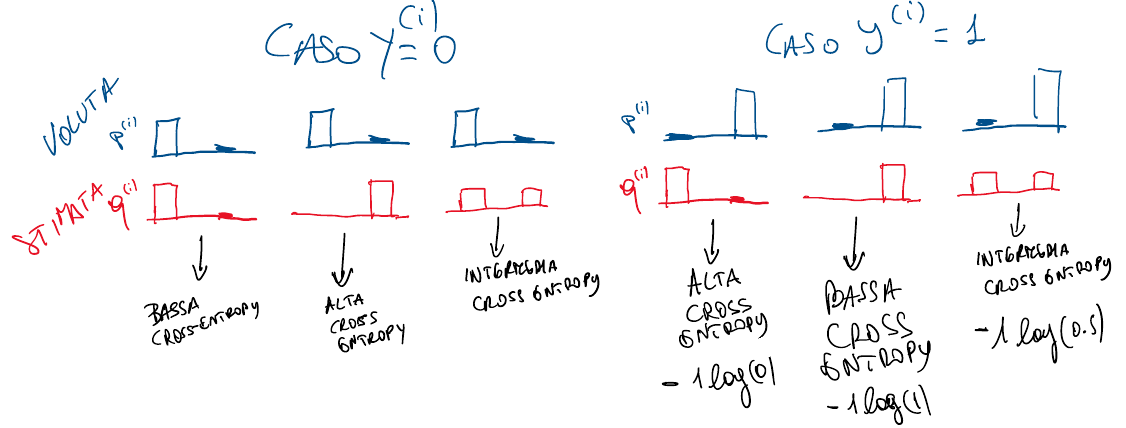
\includegraphics[width=0.8\linewidth]{images/coss-entropy2}
\end{figure}

\section{Overfitting nella classificazione}
Rischiamo di cadere in overfitting nell'utilizzo di classificatori polinomiali. Basterà usare i termini di regolarizzazione per diminuire o annullare l'impatto di alcuni termini di grado eccessivamente alto, ottenendo così:
$$
J(\vartheta) = - \frac{1}{m} \sum_{i=1}^{m}(y^{(i)}\log (h_\vartheta(x)) + (1-y^{(i)})\log (1 - h_\vartheta(x))) + \frac{\lambda}{2m}\sum_{j=1}^n\vartheta_j^2
$$ 

\begin{figure}[tbph]
	\centering
	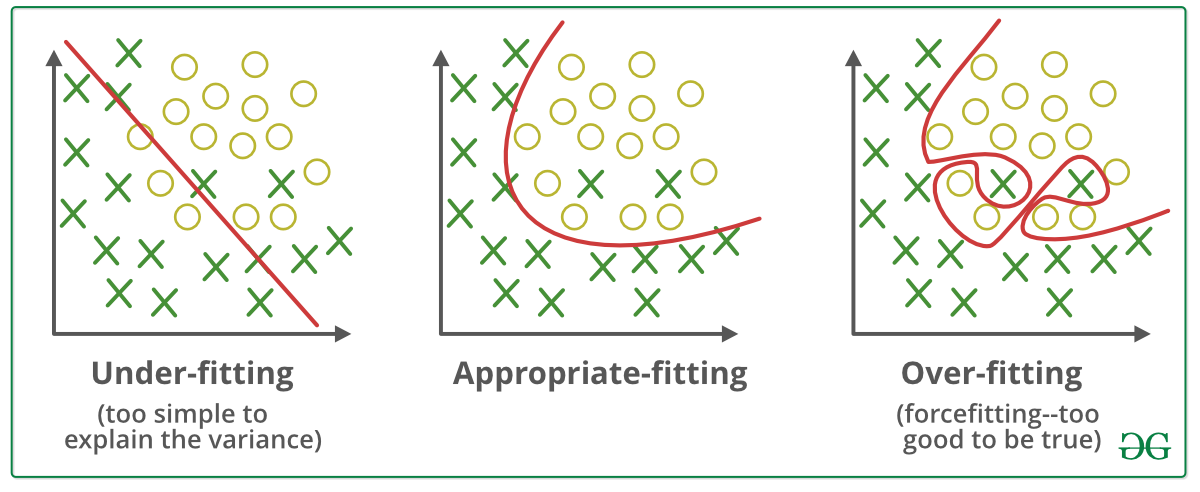
\includegraphics[width=1\linewidth]{images/underoverfitting-classification}
\end{figure}

\section{Reject Region, regione d'incertezza}

Sia nella classificazione binaria, che in quella multiclasse, è possibile osservare casi in cui la probabilità stimata che un input appartenga ad una tra le classi specificate, non superi un determinato valore di certezza. Sono dei casi limite che vanno gestiti in maniera opportuna:
\begin{enumerate}
	\item Prendere il valore con certezza più alta, se è proprio obbligatorio stabilire una classe, e il task non è particolarmente delicato.
	\item Scartare l'input. Un'opzione migliore in campi più dellicati, come quello medico.
\end{enumerate}

\begin{figure}[tbph]
	\centering
	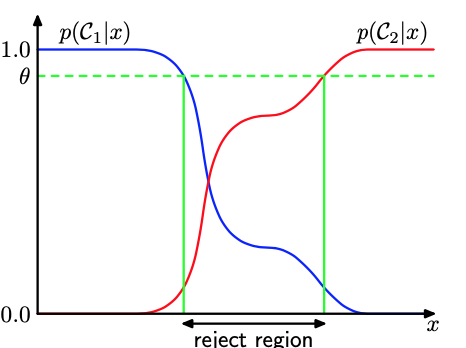
\includegraphics[width=0.47\linewidth]{images/rejection-region}
	\caption{La zona d'incertezza (in cui $P(C_1|x) \sim P(C_2|x)$)}
\end{figure}

\section{Classificazione multiclasse, approccio naive OVA e OVO}  
La classificazione multiclasse si distingue da quella binaria per il numero di classi.
Il dataset di input non avrà più etichette binarie, ma $k$ etichette. A ogni classe si associa un numero, ai fini di semplicità. 

\subsection{Metodo One vs All}
Possiamo ottenere una classificazione multiclasse da dei classificatori binari, usando la metodologia \textbf{one vs all}. Immaginiamo di avere un sistema di classificazione figure geometriche, con le classi \textit{triangolo}, \textit{quadrato }e \textit{cerchio }($c_1,c_2,c_3$).
Avremo bisogno di tre classificatori, $h_{\vartheta}^1, h_{\vartheta}^2, h_{\vartheta}^3$, capaci di misurare $P(\text{triangolo}|x), P(\text{quadrato}|x), $ $P(\text{cerchio}|x)$. Prenderemo poi l'etichetta associata al valore di probabilità più alto

$$
\hat{k} = \text{arg}\max_k h_{\vartheta}^k(\overline{x})
$$

ottenendo effettivamente una classificazione multiclasse. 

\begin{figure}[tbph]
	\centering
	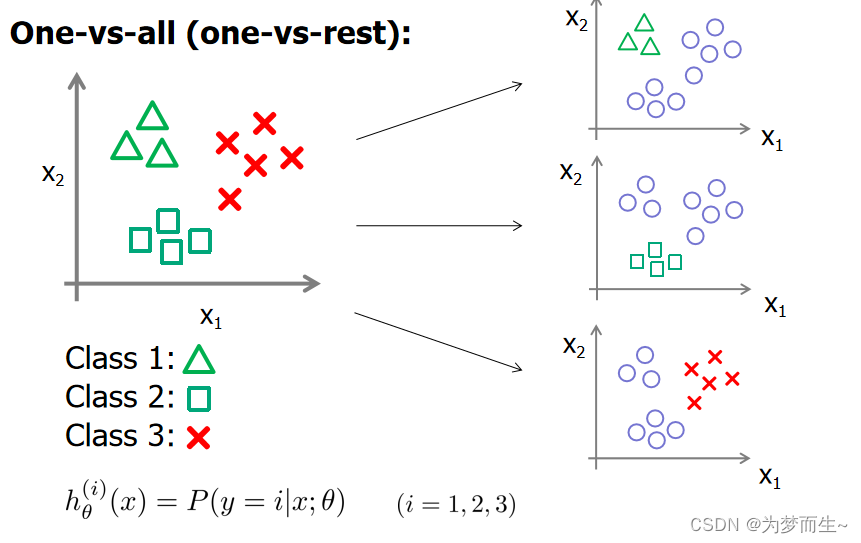
\includegraphics[width=0.8\linewidth]{images/onevsrest}
\end{figure}

Il training è effettuato sui singoli classificatori binari.
Osserviamo inoltre che, con $k$ classi:

$$
\text{Numero di classificatori richiesti in one vs all} = k 
$$

\subsection{Metodo One vs One}
In questo caso, i classificatori distinguono classi a due a due. Si fanno poi le opportune valutazioni per capire quale classe assegnare. Il numero di classificatori risulta essere più alto. Con $k$ classi abbiamo:

$$
\text{Numero di classificatori richiesti in one vs one} = \frac{k(k-1)}{2}
$$

Immaginiamo un classificatore per lo stesso problema precedentemente esposto: otteniuamo le classi $(c_1,c_2,c_3)$. Questi classificatori su coppie, daranno poi dei risultati. La classe più votata vince:
$$
c_1 \text{ vs } c_2, \quad c_2 \text{ vs } c_3, \quad c_1 \text{ vs } c_3
$$

\begin{figure}[tbph]
	\centering
	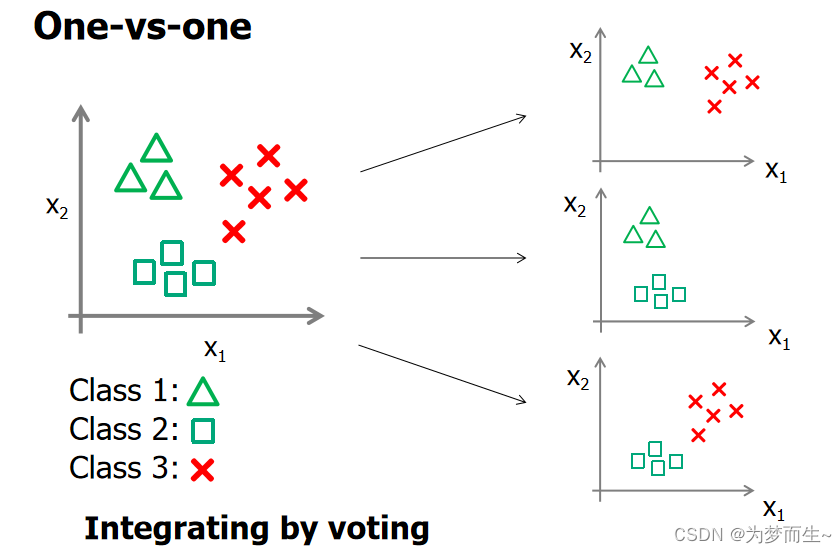
\includegraphics[width=0.75\linewidth]{images/onevsone}
\end{figure}


\subsection{Confronto tra \textit{One vs All} e \textit{One vs One}}
Il modello one vs one, per quanto più oneroso in termini di numero di classificatori binari richiesti, non presenta l'area di incertezza su tutte le classi, che invece possiamo trovare nel classificatore one vs all.

\begin{figure}[tbph]
	\centering
	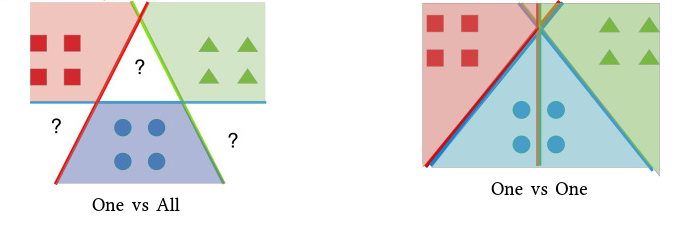
\includegraphics[width=0.75\linewidth]{images/onevsonevsonevsall}
\end{figure}

\section{Stochastic Gradient Descent}
L'algoritmo di discesa del gradiente, computa $J(\vartheta)$ su \textbf{tutti} i campioni del training set: associando al numero di campioni il valore $m$, a $d$ il numero di feature e ad $e$ le epoche di training, otteniamo un numero di operazioni complessive pari a 

$$
m \times d \times e
$$

Questo prodotto raggiunge facilmente valori molto alti. Un modo per ridurre il numero di operazioni, senza intaccare il risultato del training, e arrivare a convergenza, è l'uso della \textbf{SGD}, ossia della \textbf{discesa del gradiente stocastica}. Ad ogni iterazione del training si campiona un mini-\textbf{batch} di campioni di dimensione $b \leq m$. Questo campione è scelto randomicamente a ogni iterazione.
$$
b \times d \times e
$$

L'algoritmo deve arrivare a convergenza: se non arriva a convergenza, si ripete il campionamento e si ripete il training.

\section{Softmax - Classificazione Multiclasse}
Abbiamo quindi visto com'è possibile implementare un classificatore multiclasse utilizzando più classificatori binari. Tuttavia, questa strategia (a prescindere da OVA e OVO) presenta delle criticità:

\begin{itemize}
	\item Numero di classificatori elevato, che porta a tempi di training lunghi.
	\item Possibili aree di incertezza.
	\item Difficoltà nell'interpretare le probabilità restituite dai classificatori.
\end{itemize}

Si può ovviare a questi problemi con il modello \textbf{Softmax}, che estende la regressione logistica alla classificazione multiclasse.

\subsection{Definizione}
Sia $K$ il numero di classi da prevedere. Il modello Softmax restituisce un vettore $P_\vartheta^{(k)}$ di lunghezza $K$, in cui ogni elemento $P_\vartheta^{(i)}$ rappresenta \textbf{la probabilità} che l'input $x$ appartenga alla classe $i$. L'obiettivo è quindi, cercare di \textbf{stimare}:
\[
P_{\vartheta}^{(k)}(y=k | x) \qquad \forall k \in \{1, \ldots, K\}
\]

la somma di ogni elemento del vettore, è sempre $=1$.
\subsection{Funzione Softmax}
Partiamo dall'idea che il softmax restituisce un vettore di probabilità:
\[
h_{\vartheta}^{(c)}(x) = 
\begin{pmatrix}
P_{\vartheta}^{(1)}(y=1 | x) \\
P_{\vartheta}^{(2)}(y=2 | x) \\
\vdots \\
P_{\vartheta}^{(K)}(y=K | x)
\end{pmatrix}
= 
\frac{1}{\underbrace{\sum_{k=0}^{K-1} e^{\vartheta^{(k) T} x}}_{\text{Normalizzatore della distribuzione}}}
\cdot
\begin{pmatrix}
e^{\vartheta^{(1) T} x} \\
e^{\vartheta^{(2) T} x} \\
\vdots \\
e^{\vartheta^{(k) T} x}
\end{pmatrix}
=
\frac{e^{\vartheta^{(c) T} x}}{\sum_{k=0}^{K-1} e^{\vartheta^{(k) T} x}}
\]

\noindent
Dove $c$ è la classe di cui vogliamo calcolare la probabilità, $k$ è l'indice che scorre tutte le classi, e $\vartheta^{(k)}$ è il vettore dei parametri associati alla classe $k$.

\textbf{N.B.} Ogni classe $k$ ha il proprio vettore di parametri $\vartheta^{(k)}$ (i pesi del modello). Inoltre, una volta finito il learning del modello, la somma delle probabilità restituite dal softmax sarà sempre pari a 1 ($\displaystyle\sum_{k=1}^{K} P_{\vartheta}^{(k)}(y=k | x) = 1$).

\subsection{Funzione di Costo}
La funzione di costo del softmax è una funzione chiamata Cross Entropy Loss. Prima di poter definire la funzione di costo, definiamo una variabile ausiliaria \(1\{\text{proposizione}\} \) che vale 1 se la proposizione è vera, 0 altrimenti.
La funzione di costo del softmax è quindi:
\[
J(\vartheta) = 
- \frac{1}{m} 
\left[
\sum_{i=1}^{m} \sum_{c=1}^{K} 1\{y^{(i)} = c\} \log P_{\vartheta}^{(c)}(y=c | x^{(i)})
\right]
+
\underbrace{\frac{\lambda}{2} \sum_{c=1}^{K} \sum_{j=1}^{n} (\vartheta_j^{(c)})^2}_{\text{Termine di regolarizzazione}}
\]

\noindent
Dove il termine di regolarizzazione serve a prevenire l'overfitting del modello.

\subsection{Obiettivo di Learning}
L'obiettivo di learning è quello di minimizzare la funzione di costo, trovando i parametri ottimali \(\vartheta\):
\[
\vartheta = \arg \min_{\vartheta} J(\vartheta)
\]

Ovvero , trovare i parametri che minimizzano la distanza tra la distribuzione di probabilità predetta dal modello e la distribuzione di probabilità reale (ground truth).

Per fare questo possiamo usare la discesa del gradiente, per cui abbiamo bisogno della derivata parziale della funzione di costo rispetto ai parametri \(\vartheta_j^{(c)}\):
\[
\frac{\partial J(\vartheta)}{\partial \vartheta_j^{(c)}}
=
- \frac{1}{m}
\sum_{i=1}^{m}
\left[
\left(1\{y^{(i)} = c\} - P_{\vartheta}^{(c)}(y=c | x^{(i)})\right)
x_j^{(i)}
\right]
+
\underbrace{\lambda \vartheta_j^{(c)}}_{\text{Termine di regolarizzazione}}
\]

E da questa, aggiorniamo i pesi \(\vartheta_j^{(c)}\) utilizzando la regola di aggiornamento della discesa del gradiente:
\[
\vartheta_j^{(c)} \leftarrow \vartheta_j^{(c)} - \alpha \frac{\partial J(\vartheta)}{\partial \vartheta_j^{(c)}}, \qquad \forall j \in [0, n], \quad \forall c \in [0, K-1]
\]

\subsection{Proprietà del Softmax}\label{sec:proprieta_softmax}
Il modello softmax è \textbf{overparametrizzato}: per ogni ipotesi che potrebbe essere fatta sui dati, esistono infinite combinazioni di parametri che a partire dal vettore di feature $X \in \mathbb{R}^n$ producono la stessa predizione nel vettore di probabilità $Y$.

\noindent
Per dimostrarlo, partiamo da:
\begin{align*}
h_{\vartheta}^{(c)}(x) 
&=\dfrac{e^{\vartheta^{(c)\!\top} x}}
        {\displaystyle\sum_{k=0}^{K-1} e^{\vartheta^{(k)\!\top} x}}
        && \text{Formula del Softmax} \\[4pt]
&=\dfrac{e^{(\vartheta^{(c)}-\psi)^{\!\top} x}}
        {\displaystyle\sum_{k=0}^{K-1} e^{(\vartheta^{(k)}-\psi)^{\!\top} x}}
        && \text{Sottraiamo lo stesso $\psi$} \\[4pt]
&=\dfrac{e^{\vartheta^{(c)\!\top} x}\,e^{-\psi^{\!\top} x}}
        {\displaystyle\sum_{k=0}^{K-1} e^{\vartheta^{(k)\!\top} x}\,e^{-\psi^{\!\top} x}}
        && \text{Separiamo gli esponenziali} \\[4pt]
&=\dfrac{e^{\vartheta^{(c)\!\top} x}}
        {\displaystyle\sum_{k=0}^{K-1} e^{\vartheta^{(k)\!\top} x}}
        && \text{Si cancella il fattore comune $e^{-\psi^{\!\top} x}$}
\end{align*}

\noindent
Dove $\psi \in \mathbb{R}^n$ è un vettore arbitrario. Quindi, sottraendo lo stesso vettore $\psi$ da tutti i vettori di parametri $\vartheta^{(k)}$, otteniamo gli stessi valori di probabilità predetti dal modello, perciò esistono infinite combinazioni di parametri che producono la stessa predizione.

\paragraph{Nota.} Può essere trovato un approfondimento di questa parte nell'appendice \ref{chap:approfondimenti_teorici} alla sezione \ref{sec:softmax_generalizzazione_logistica}.

\subsection{Rete neurale Softmax}
Il softmax può essere visto come un particolare tipo di rete neurale:
\begin{figure}[htbp]
	\centering
	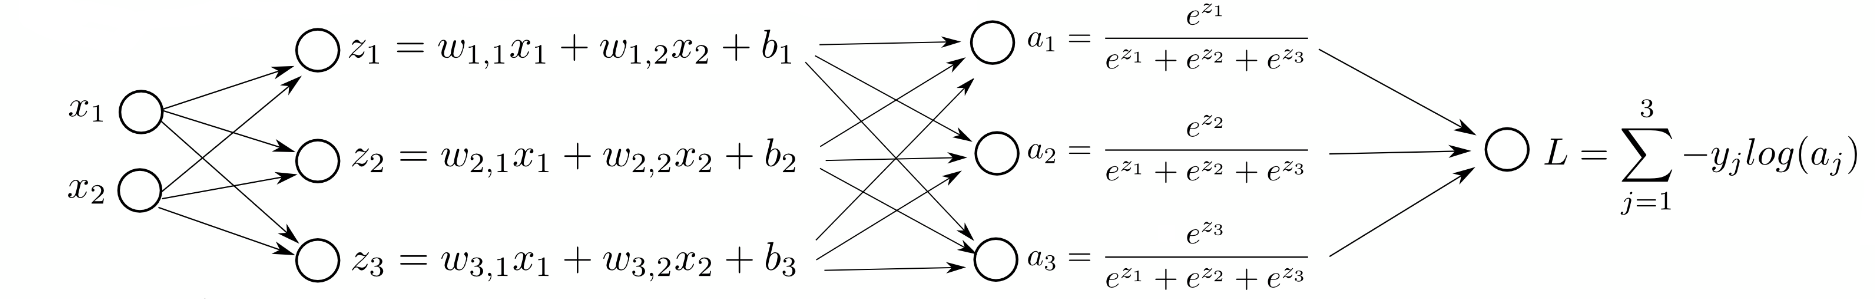
\includegraphics[width=\textwidth]{images/softmax_neural_network.png}
	\caption{Flusso della regressione softmax con due ingressi e tre classi: dai logit
	$z_i = w_{i,1}x_1 + w_{i,2}x_2 + b_i$ alle probabilità
	$a_i=\frac{e^{z_i}}{\sum_{k=1}^{3} e^{z_k}}$, fino alla loss a entropia incrociata
	$L = \sum_{j=1}^{3} -y_j \log(a_j)$.}	
	\label{fig:softmax_neural_network}
\end{figure}

\subsection{Funzione di Loss}
La funzione di Loss usata nel softmax normalmente è una variante di \textbf{cross entropy loss}. Il softmax, infatti, restituisce un vettore di probabilità, e la cross entropy loss misura la distanza tra questa distribuzione di probabilità e la distribuzione di probabilità reale (ground truth).

Si possono usare alternative, in particolare la \textbf{Hinge Loss} trasforma la classificazione multiclasse in un problema di massimizzazione del margine tra le classi, come nelle SVM. La Hinge Loss è definita come:
\[
\text{Loss}(h_\vartheta(x), y) = \sum_{i \neq y} \max(0, h_\vartheta(x)_i - h_\vartheta(x)_y + \Delta)
\]

In questo contesto massimizzare il margine significa cercare di rendere la probabilità della classe corretta $h_\vartheta(x)_y$ significativamente maggiore rispetto alle probabilità delle classi errate $h_\vartheta(x)_i$, con un margine di sicurezza $\Delta$.

\section*{Riferimenti}
Il materiale di questo capitolo comprende:
\begin{itemize}
	\item Materiale visto a lezione.
\end{itemize}